Next, we measured the file cache size. Our hypothesis is that the file cache size is dynamic and that it depends on the amount of free memory available to the system since it would not make sense for the system to keep a lot of free pages around when they could be used to speed up repeated reads.

To check our hypothesis, we designed two controlled experiments with different amounts of free memory available to the system. One experiment runs with most of the memory unused. In the other experiment, we allocate a huge array and fill it with random data to avoid page sharing effects. We call this array \emph{balloon}. We used a 10GB balloon in the host environment and a 3GB balloon in the virtual machine since they had different RAM sizes.

Each experiment consists of four repeated sequential reads of varying size. We measure throughput on the last three reads. If the read size is smaller than the file cache size, the data accessed in repeated reads reside in the cache, making repeated reads very fast. As soon as the size of our reads exceeds the cache size, we expect to see huge decrease in total throughput since some of the repeated reads will need to go to disk and wait for I/O. Figure \ref{fig:p3pseudo} shows the pseudocode of the experiments. We used 20MB for the buffer size, guided by insight from Section \ref{sec:p1}. In the virtual environment we had to be careful to avoid the effects of the host file cache so we flushed the host file cache before every read.

\begin{figure}
\begin{algorithmic}
\STATE clear cache
\IF {ballooning enabled}
\STATE allocate huge array
\STATE fill the array with random data
\ENDIF
\STATE $size \leftarrow$ {sequential read size}
\STATE $file \leftarrow$ {huge file filled with random data}
\STATE $buffer\_size \leftarrow$ 20MB
\STATE flush the cache
\STATE read first $size$ bytes of $file$
\FOR{$i = 0$ to $3$}
\IF {running in VM}
\STATE clear host file cache
\ENDIF
\STATE open $file$
\WHILE{total bytes read $< size$}
\STATE start\_timer
\STATE read next $buffer\_size$ bytes
\STATE end\_timer and save the result
\ENDWHILE
\STATE close $file$
\ENDFOR
\STATE report average of all timers divided by $buffer\_size$
\end{algorithmic}
\caption{Function used to measure file cache size}
\label{fig:p3pseudo}
\end{figure}

Figure \ref{fig:p3graph} shows the repeated read throughput for each measured sequential read size. We observe the expected behavior for all four cases. First, we see a sharp decrease in throughput after a certain point: 6GB for VM with ballooning, 8GB for the VM without ballooning, 12GB for the host with ballooning, and 22GB for the host without ballooning. We attribute this effect to read sizes getting bigger than the file cache. Next, we observe a smaller file cache size when running experiments with ballooning, which proves our hypothesis that the file cache size is dynamic and depends on the amount of free memory available to the system. The difference between the points of sharp decline in throughput for the cases with and without ballooning -- 2GB for the VM and 10GB for the host -- is roughly the size of the balloon. We attribute the disparity for the VM case due to the granularity of our measurement, which rounds down to the nearest GB. It is interesting to note that the kernel did not decide to swap out the balloon array and increase the file cache size, even though it would speed up execution of our program. However, we can not make any inferences about the general policy of swapping out memory to increase file cache size. 

\begin{figure}[t!]
	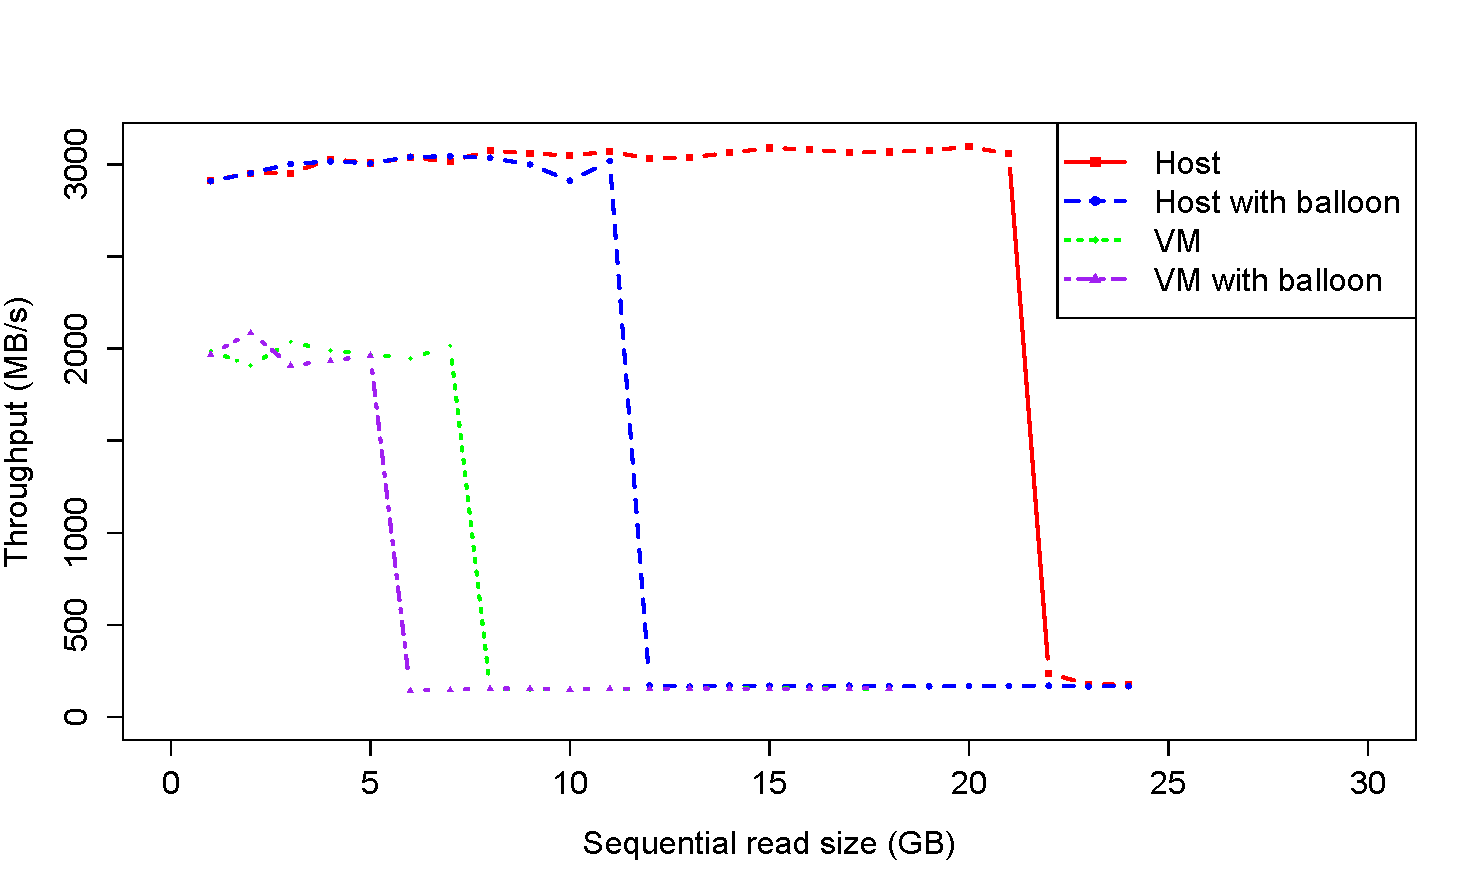
\includegraphics[width=0.5\textwidth]{./figures/p3.pdf}
	\caption{Repeated sequential read throughput. Horizontal axis shows size of repeated sequential read and vertical axis shows throughput. Throughput was measured in four environments: Host with a lot of free memory, Host with 10GB balloon, Virtual Machine with a lot of free memory and Virtual Machine with 3GB balloon.}
	\label{fig:p3graph}
\end{figure}
